% Provenance (never printed): cycle 3 "La planete Terre" (natural phenomena
% and the risks they bring: storms, floods, droughts, earthquakes, eruptions;
% warnings and the right behaviour); see sources/book1/PROVENANCE.md.
% Book 1, grade 5, chapter 3.
\chapter{الأخطار الطبيعية}\label{ch:g5:natural-hazards}

إنه مساء الجمعة. في المذياع، تتوقف الموسيقى ويقرأ صوت هادئ
تحذيرًا: \omterm{def:g5:natural-hazards:storm}{عاصفة} قوية ستبلغ \omterm{def:g1:landscapes-around-us:water}{الساحل} الليلة، برياح قوية جدًا \omterm{def:g4:clouds-rain-snow:precipitation}{ومطر} غزير.
ويُطلب من الناس أن يبقوا في بيوتهم من الساعة التاسعة،
وأن يربطوا أو يُدخلوا كل ما قد تحمله الريح بعيدًا.

تبدأ أسرة لينا العمل. يُدخل أبوها كراسي الحديقة والطاولة
إلى السقيفة. وتتأكد أمها أن المصابيح اليدوية تعمل وتضع
بطاريات احتياطية على طاولة المطبخ. وتملأ لينا قارورتين كبيرتين
بالماء. وعند التاسعة، يكون الجميع في الداخل، والريح تعوي
منذ الآن.

\begin{omfigure}

\includegraphics[width=0.5\linewidth]{images/book1/ai/g5-radio-warning.jpg}

{\small أسرة تستمع إلى تحذير من \omterm{def:g5:natural-hazards:storm}{عاصفة} في المذياع، والمصابيح اليدوية
والبطاريات الاحتياطية جاهزة.}
\end{omfigure}

\begin{recall}
\omterm{def:g4:volcanoes-earthquakes-first-look:volcano}{البركان} قد يثور، فيقذف \omterm{def:g4:volcanoes-earthquakes-first-look:eruption}{حممًا} ورمادًا وغازًا؛ \omterm{def:g4:volcanoes-earthquakes-first-look:earthquake}{والزلزال} اهتزاز مفاجئ
للأرض؛ وأثناء \omterm{def:g4:volcanoes-earthquakes-first-look:earthquake}{الزلزال}، ننبطح ونحتمي ونتمسك
(\cref{ch:g4:volcanoes-earthquakes-first-look}). \omterm{def:g1:landscapes-around-us:water}{والنهر} الذي يتلقى من الماء
أكثر مما يتسع له مجراه يغمر \omterm{def:g5:water-shapes-the-land:flood}{سهله الفيضي}
(\cref{ch:g5:water-shapes-the-land}). ولكل مكان مناخه، والنطاقات
الحارة والمعتدلة والباردة تدور حول \omterm{def:g3:continents-and-oceans:globe}{مجسم الكرة الأرضية}
(\cref{ch:g5:weather-and-climate}).
\end{recall}

\section{ما الخطر الطبيعي}

الطبيعة ليست هادئة دائمًا. فالريح قد تهب بقوة تكفي لكسر
الأشجار، \omterm{def:g1:landscapes-around-us:water}{والأنهار} قد تفيض، والأرض قد تهتز. وهذه الأحداث جزء من
طريقة عمل الأرض: فقد حدثت قبل وجود الناس بزمن طويل، وستظل
تحدث.

\begin{definition}[الخطر الطبيعي]\label{def:g5:natural-hazards:hazard}
\emph{الخطر الطبيعي}\index{خطر طبيعي} حدث طبيعي قد
يؤذي الناس أو يتلف ما بنوه: \omterm{def:g5:natural-hazards:storm}{عاصفة}، \omterm{def:g5:water-shapes-the-land:flood}{فيضان}، \omterm{def:g5:natural-hazards:drought}{جفاف}،
\omterm{def:g4:volcanoes-earthquakes-first-look:earthquake}{زلزال}، \omterm{def:g4:volcanoes-earthquakes-first-look:eruption}{ثوران} بركاني، \omterm{def:g5:natural-hazards:landslide}{انزلاق أرضي}{\ldots}
\end{definition}

نستطيع أن نصنف \omterm{def:g5:natural-hazards:hazard}{الأخطار الطبيعية} بحسب مصدرها: من الهواء، أو من
الماء، أو من الأرض.

\begin{omfigure}
\begin{tikzpicture}[font=\small, box/.style={draw, rounded corners=3pt,
    minimum width=4.2cm, minimum height=0.9cm, align=center}]
  \node[box, fill=cyan!15, font=\small\bfseries] (A) at (9.6,0) {من الهواء};
  \node[box, fill=blue!15, font=\small\bfseries] (W) at (4.8,0) {من الماء};
  \node[box, fill=brown!25, font=\small\bfseries] (G) at (0,0) {من الأرض};
  \node[align=center, anchor=north] at (9.6,-0.7) {العواصف\\الأعاصير المدارية\\موجات الحر\\الجفاف};
  \node[align=center, anchor=north] at (4.8,-0.7) {الفيضانات\\من الأنهار\\من المطر الغزير\\من البحر في العاصفة};
  \node[align=center, anchor=north] at (0,-0.7) {الزلازل\\الثورانات البركانية\\الانزلاقات الأرضية};
  \node[draw, rounded corners=3pt, fill=gray!10, font=\small\bfseries,
    minimum width=5cm, minimum height=0.8cm] (N) at (4.8,1.5) {الأخطار الطبيعية};
  \draw[->] (N.south) -- (A.north);
  \draw[->] (N.south) -- (W.north);
  \draw[->] (N.south) -- (G.north);
\end{tikzpicture}

{\small \omterm{def:g5:natural-hazards:hazard}{الأخطار الطبيعية}، مصنفة بحسب مصدرها.}
\end{omfigure}

\section{أخطار من الهواء}

\begin{definition}[العاصفة]\label{def:g5:natural-hazards:storm}
\emph{العاصفة}\index{عاصفة} وقت من الريح القوية جدًا، يرافقه عادة
\omterm{def:g4:clouds-rain-snow:precipitation}{مطر} غزير أو \omterm{def:g4:clouds-rain-snow:precipitation}{ثلج}، وأحيانًا رعد وبرق.
\end{definition}

\omterm{def:g5:natural-hazards:storm}{العاصفة} القوية تكسر الأغصان، وتسقط الأشجار، وتنتزع القرميد عن السطوح،
وقد تقذف كراسي الحديقة عبر النوافذ. وعلى \omterm{def:g1:landscapes-around-us:water}{الساحل}، تكدّس ريحها
\omterm{def:g2:water-on-earth:ocean}{البحر} على الشاطئ وترسل أمواجًا هائلة فوق الأسوار البحرية.

أقوى العواصف على الأرض تتكون فوق البحار المدارية الدافئة. إنها
عواصف هائلة دوّارة: فهي تبدو من الفضاء كأنها لولب عملاق من
\omterm{def:g4:clouds-rain-snow:cloud}{السحب}، في وسطه ثقب هادئ صافٍ، هو العين. وحول العين
تهب أقوى الرياح. ولهذا النوع نفسه من العواصف أسماء مختلفة في
محيطات مختلفة: فيسمى \emph{هاريكين} في شمال الأطلسي وفي
شرق \omterm{def:g2:water-on-earth:ocean}{المحيط} الهادئ، و\emph{تيفون} في شمال غرب \omterm{def:g2:water-on-earth:ocean}{المحيط} الهادئ،
و\emph{إعصارًا مداريًا} في جنوب \omterm{def:g2:water-on-earth:ocean}{المحيط} الهادئ وفي \omterm{def:g2:water-on-earth:ocean}{المحيط} الهندي.
% ledger: noaa:cyclone-names

\begin{omfigure}
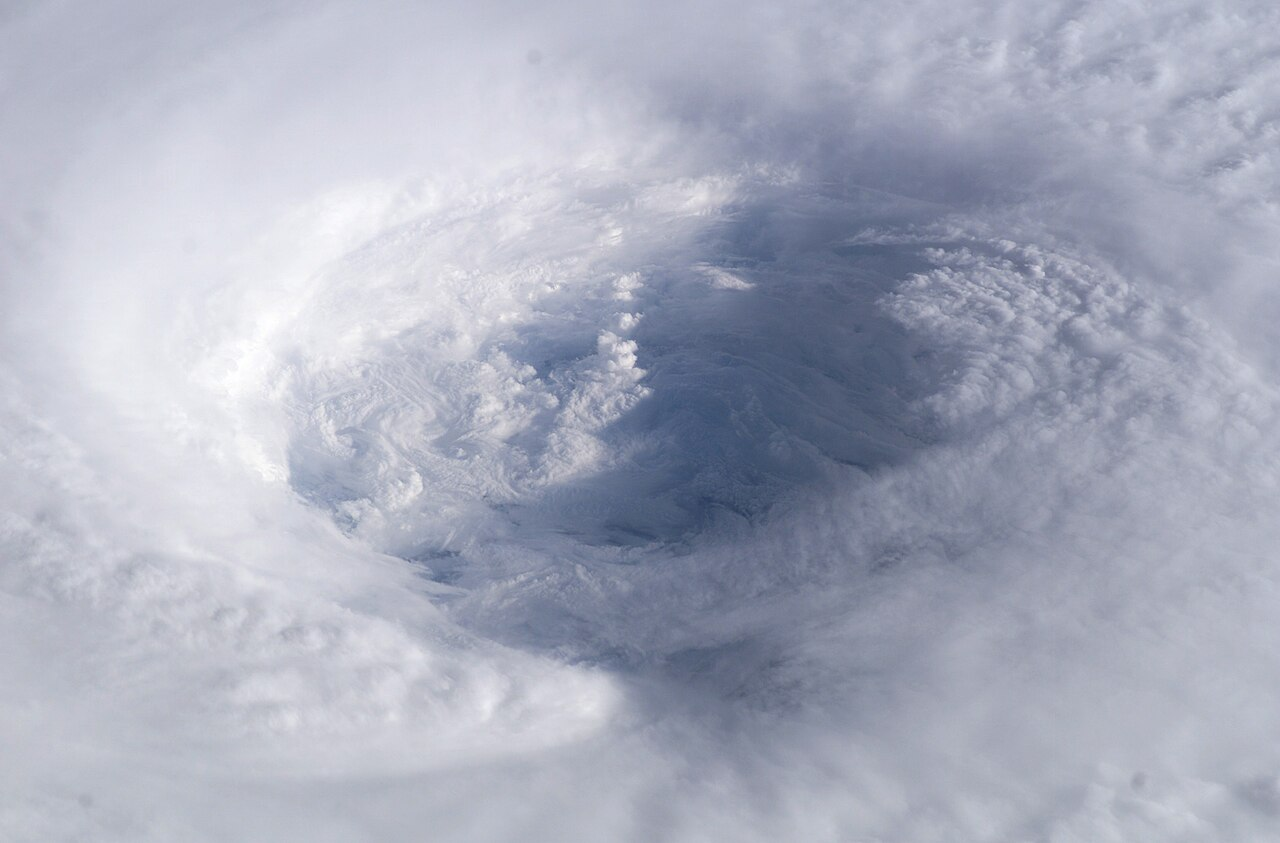
\includegraphics[width=0.5\linewidth]{images/book1/g5-hurricane-isabel-iss.jpg}

{\small نظرة من الأعلى إلى عين الإعصار إيزابيل، فوق \omterm{def:g2:water-on-earth:ocean}{المحيط} الأطلسي
في سبتمبر 2003، من محطة الفضاء الدولية: جدار من
\omterm{def:g4:clouds-rain-snow:cloud}{السحب} حول مركز أهدأ. الصورة: NASA (ملك عام).}
% ledger: nasa:isabel-iss
\end{omfigure}

بعض الأخطار الآتية من الهواء بطيئة صامتة. ف\emph{موجة الحر}
فترة من أيام وليال عدة أشد حرًا بكثير من المعتاد. وهي
خطرة قبل كل شيء على كبار السن جدًا والرضّع والمرضى.

\begin{definition}[الجفاف]\label{def:g5:natural-hazards:drought}
\emph{الجفاف}\index{جفاف} فترة طويلة، من أشهر بل من سنين،
يسقط فيها من \omterm{def:g4:clouds-rain-snow:precipitation}{المطر} أقل بكثير من المعتاد في ذلك المكان. فتجف التربة، وتنكمش
\omterm{def:g1:landscapes-around-us:water}{الأنهار} \omterm{def:g1:landscapes-around-us:water}{والبحيرات}، وتذبل المحاصيل وتموت.
\end{definition}

\omterm{def:g5:natural-hazards:drought}{الجفاف} يزحف ببطء: لا أحد يستطيع أن يقول في أي يوم يبدأ. لكن
\omterm{def:g5:natural-hazards:drought}{الجفاف} الطويل قد يترك المزارعين بلا حصاد والمدن في نقص من الماء.

\begin{omfigure}
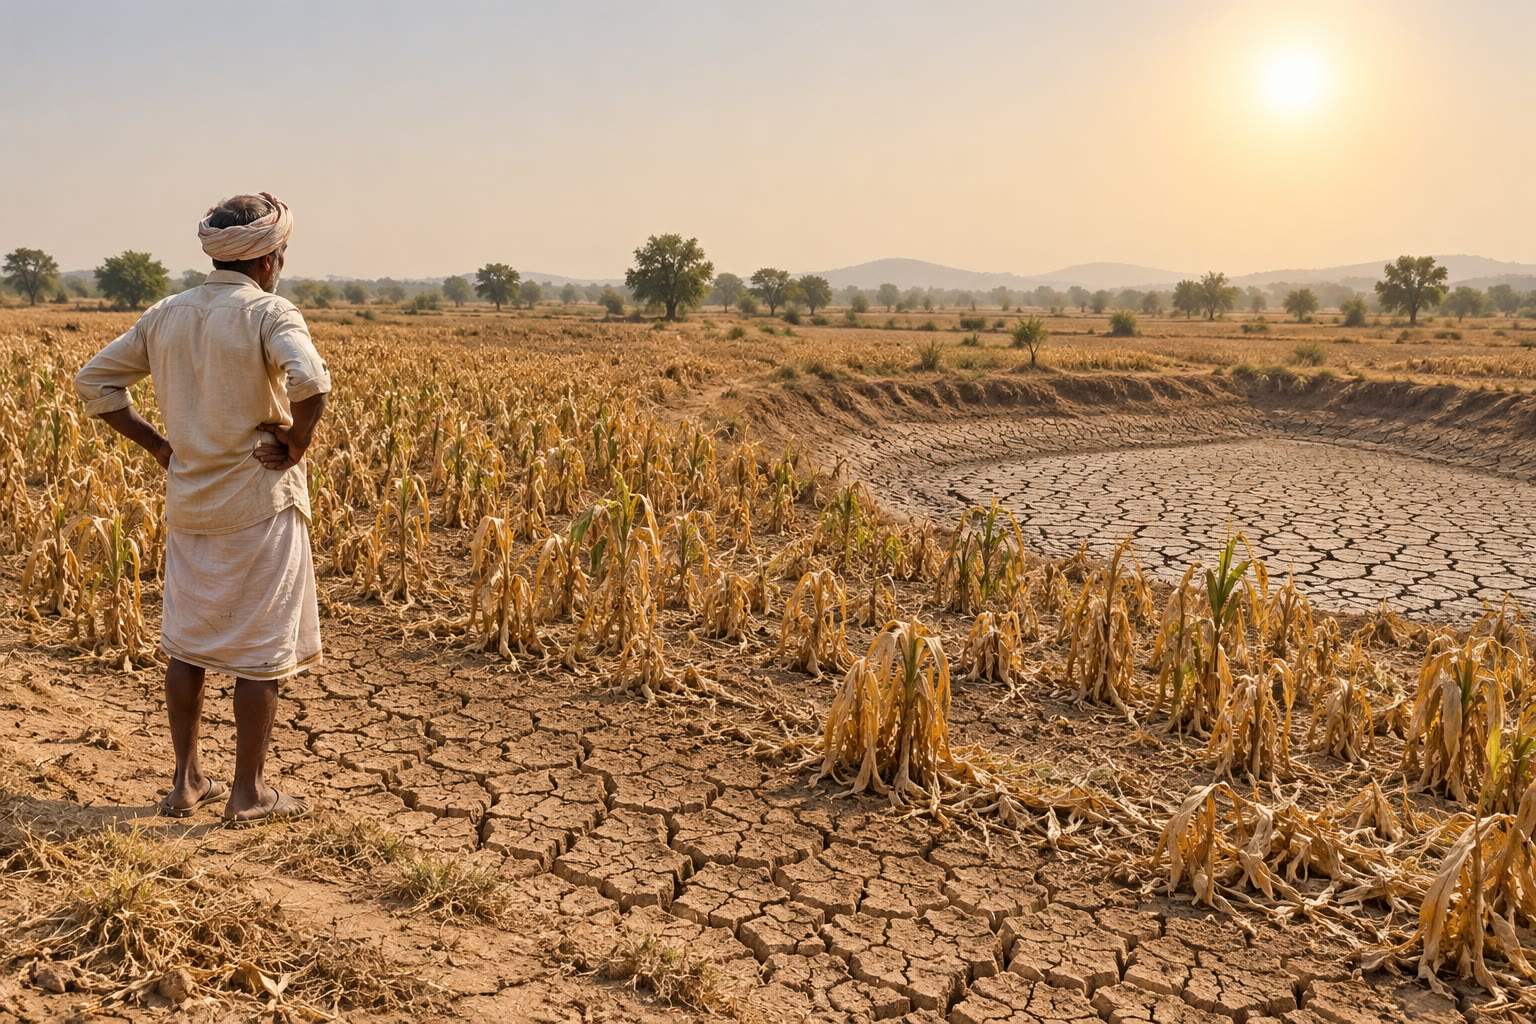
\includegraphics[width=0.42\linewidth]{images/book1/ai/g5-drought-field.jpg}

{\small حقل في \omterm{def:g5:natural-hazards:drought}{جفاف} طويل: الأرض متشققة، والمحاصيل
صفراء، والبركة قد جفت.}
\end{omfigure}

\section{أخطار من الماء}

أنت تعرف من قبل \omterm{def:g5:water-shapes-the-land:flood}{فيضانات} \omterm{def:g1:landscapes-around-us:water}{الأنهار} (\cref{ch:g5:water-shapes-the-land}).
فبعد أيام من \omterm{def:g4:clouds-rain-snow:precipitation}{المطر}، أو حين يذوب \omterm{def:g4:clouds-rain-snow:precipitation}{الثلج} سريعًا، يرتفع \omterm{def:g1:landscapes-around-us:water}{النهر} فوق
ضفتيه ويغطي \omterm{def:g5:water-shapes-the-land:flood}{سهله الفيضي}. وبعض \omterm{def:g5:water-shapes-the-land:flood}{الفيضانات} يأتي سريعًا جدًا: فوابل
عنيف من \omterm{def:g4:clouds-rain-snow:precipitation}{المطر} على واد شديد الانحدار قد يحوّل جدولًا هادئًا إلى سيل هادر
في أقل من ساعة. وبعضها يأتي من \omterm{def:g2:water-on-earth:ocean}{البحر}، حين تدفع \omterm{def:g5:natural-hazards:storm}{العاصفة} الماء
إلى \omterm{def:g1:landscapes-around-us:water}{ساحل} منخفض.

\section{أخطار من الأرض}

أنت تعرف من قبل \omterm{def:g4:volcanoes-earthquakes-first-look:earthquake}{الزلازل} \omterm{def:g4:volcanoes-earthquakes-first-look:eruption}{والثورانات} البركانية
(\cref{ch:g4:volcanoes-earthquakes-first-look}). وهناك خطر ثالث
من الأرض، وكثيرًا ما يكون الماء هو ما يطلقه.

\begin{definition}[الانزلاق الأرضي]\label{def:g5:natural-hazards:landslide}
\emph{الانزلاق الأرضي}\index{انزلاق أرضي} كتلة من \omterm{def:g3:stones-pebbles-sand:rock}{الصخر} أو التراب أو \omterm{def:g3:stones-pebbles-sand:sand}{الوحل}
تنزلق أو تسقط فجأة على منحدر.
\end{definition}

المنحدر الشديد الذي تشبعه الأمطار الطويلة يصير ثقيلًا زلقًا، وقد
ينهار دفعة واحدة. \omterm{def:g4:volcanoes-earthquakes-first-look:earthquake}{والزلزال} أيضًا قد يزعزع منحدرًا. \omterm{def:g5:natural-hazards:landslide}{والانزلاق الأرضي}
قد يطمر طريقًا، أو يسد نهرًا، أو يجرف بيوتًا.

\begin{omfigure}
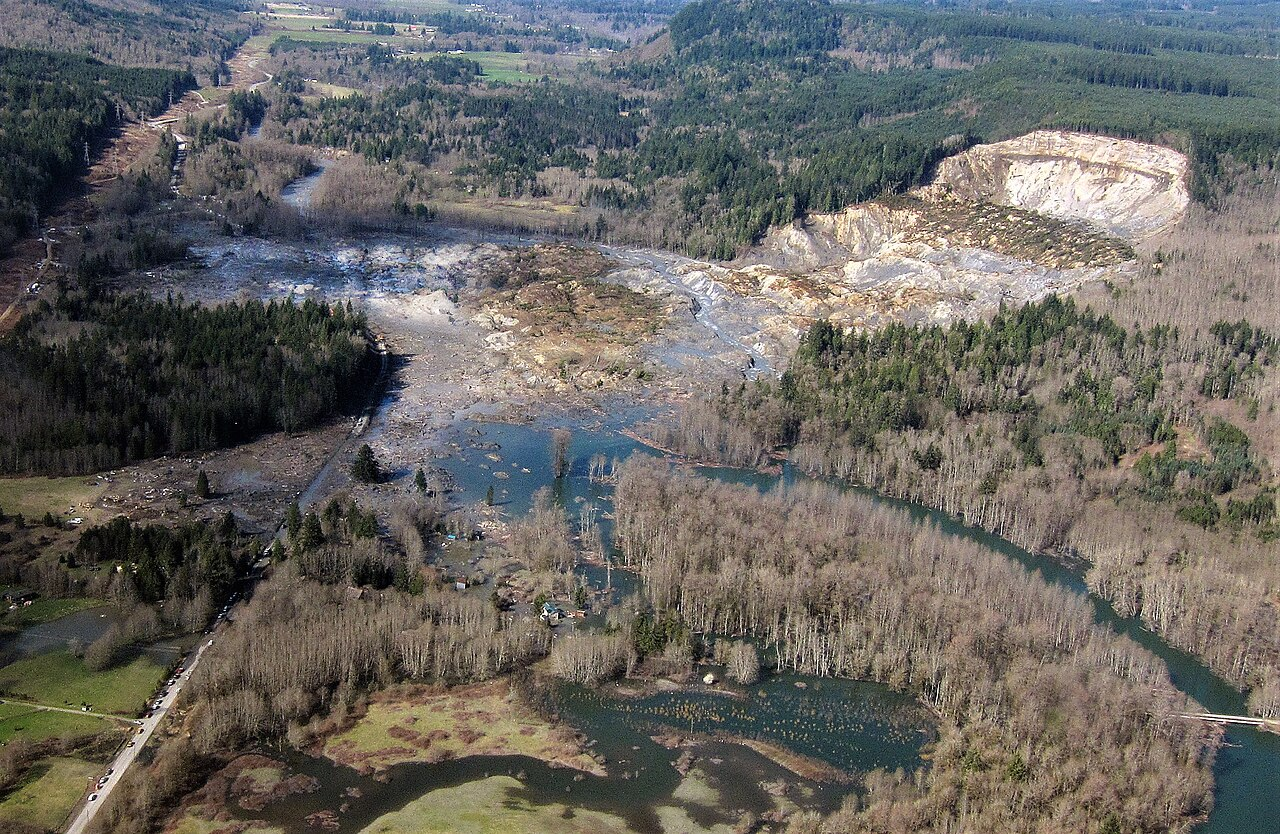
\includegraphics[width=0.6\linewidth]{images/book1/g5-landslide-washington.jpg}

{\small \omterm{def:g5:natural-hazards:landslide}{انزلاق أرضي} كبير في ولاية واشنطن، في الولايات المتحدة، عام
2014، كما يُرى من طائرة. انهار سفح التل إلى اليمين؛ وانتشر وحله
عبر \omterm{def:g1:landscapes-around-us:landform}{الوادي} كله، فغطى طريقًا وسد
\omterm{def:g1:landscapes-around-us:water}{النهر}، الذي غمر الغابة في أعلى المجرى. الصورة: مارك ريد، هيئة المسح
الجيولوجي الأمريكية USGS (ملك عام).}\label{fig:g5:natural-hazards:landslide}
% ledger: usgs:oso-aerial
\end{omfigure}

\section{من الخطر إلى الكارثة}

\omterm{def:g5:natural-hazards:storm}{عاصفة} فوق \omterm{def:g2:water-on-earth:ocean}{المحيط} المفتوح، \omterm{def:g4:volcanoes-earthquakes-first-look:earthquake}{وزلزال} في \omterm{def:g5:weather-and-climate:desert}{صحراء} خالية، \omterm{def:g5:water-shapes-the-land:flood}{وفيضان} في
واد لا يسكنه أحد: هذه \omterm{def:g5:natural-hazards:hazard}{أخطار طبيعية}، لكنها لا تؤذي
أحدًا. والأحداث نفسها تصير خطرة حين تضرب حيث يعيش الناس.

\begin{definition}[الكارثة الطبيعية]\label{def:g5:natural-hazards:disaster}
تقع \emph{الكارثة الطبيعية}\index{كارثة طبيعية} حين يضرب \omterm{def:g5:natural-hazards:hazard}{خطر
طبيعي} مكانًا يعيش فيه الناس ويُحدث أذى كبيرًا: فيُصاب الناس
أو يموتون، وتُدمَّر البيوت، وتنقطع الطرق والماء والكهرباء.
\end{definition}

\begin{omfigure}
\begin{tikzpicture}[x=1cm, y=1cm, font=\scriptsize]
  \foreach \dx/\title in {0/{الفيضان في واد خالٍ\\خطر طبيعي},
                          7.6/{الفيضان نفسه في قرية\\كارثة طبيعية}} {
    \begin{scope}[xshift=\dx cm]
      % valley sides
      \fill[green!25!brown!30] (0,0) -- (0,2.6) -- (0.4,2.6) -- (1.2,1.0) -- (5.6,1.0)
        -- (6.4,2.6) -- (6.8,2.6) -- (6.8,0) -- cycle;
      \draw[gray!60!black] (0,2.6) -- (0.4,2.6) -- (1.2,1.0) -- (5.6,1.0) -- (6.4,2.6) -- (6.8,2.6);
      % flood water over the whole valley floor
      \fill[blue!30, opacity=0.8] (1.05,1.2) -- (5.75,1.2) -- (5.6,1.0) -- (1.2,1.0) -- cycle;
      \fill[blue!30, opacity=0.8] (1.05,1.2) rectangle (5.75,1.5);
      \draw[blue!60!black] (0.95,1.5) -- (5.85,1.5);
      \node[align=center, anchor=north] at (3.4,-0.1) {\title};
    \end{scope}
  }
  % trees in the empty valley
  \foreach \x in {1.7,2.6,4.4,5.1} {
    \draw[brown!60!black, line width=1pt] (\x,1.0) -- (\x,1.75);
    \fill[green!50!black] (\x,1.95) circle (0.25);
  }
  % houses in the village valley
  \begin{scope}[xshift=7.6cm]
    \foreach \x in {1.6,2.5,3.4,4.3,5.1} {
      \fill[white, draw=black] (\x-0.3,1.0) rectangle (\x+0.3,1.65);
      \fill[red!60!black] (\x-0.38,1.65) -- (\x,2.0) -- (\x+0.38,1.65) -- cycle;
      \fill[blue!30, opacity=0.8] (\x-0.3,1.0) rectangle (\x+0.3,1.5);
    }
    % one house on the high ground, dry
    \fill[white, draw=black] (6.45,2.6) rectangle (6.77,2.95);
    \fill[red!60!black] (6.40,2.95) -- (6.61,3.2) -- (6.82,2.95) -- cycle;
  \end{scope}
\end{tikzpicture}

{\small \omterm{def:g5:water-shapes-the-land:flood}{الفيضان} نفسه مرتين. في \omterm{def:g1:landscapes-around-us:landform}{الوادي} الخالي لا يؤذي أحدًا؛ وحيث
بُنيت قرية في \omterm{def:g5:water-shapes-the-land:flood}{السهل الفيضي}، يملأ البيوت. والبيت
المبني على الأرض المرتفعة يبقى جافًا.}
\end{omfigure}

لا نستطيع أن نوقف \omterm{def:g5:natural-hazards:storm}{عاصفة} أو \omterm{def:g4:volcanoes-earthquakes-first-look:earthquake}{زلزالًا}. لكننا نستطيع أن نفعل الكثير
لنمنع الخطر من أن يصير كارثة: أن نبني بعيدًا عن \omterm{def:g1:landscapes-around-us:landform}{السهول} الفيضية
وعن أسفل المنحدرات غير المستقرة، وأن نجعل المباني متينة، وأن نراقب \omterm{def:g1:watching-the-weather:weather}{الطقس}
والأرض، وأن نحذر الناس في الوقت المناسب، وأن نعلّم الجميع ما يجب فعله.

\subsection*{التحذيرات}

مصالح الأرصاد الجوية تراقب السماء ليلًا ونهارًا. فحين تقترب \omterm{def:g5:natural-hazards:storm}{عاصفة} أو موجة حر أو
\omterm{def:g5:water-shapes-the-land:flood}{فيضان}، ترسل تحذيرات عبر المذياع والتلفزيون والهاتف
والإنترنت. وكثير من البلدان يستعمل الألوان، من الأهدأ إلى الأشد
خطورة.

\begin{omfigure}
\begin{tikzpicture}[font=\small, wstep/.style={draw=black!60, minimum width=2.6cm,
    minimum height=0.8cm, font=\small\bfseries, rounded corners=2pt}]
  \node[wstep, fill=green!45] (g) at (0,0) {أخضر};
  \node[wstep, fill=yellow!60] (y) at (0.6,0.95) {أصفر};
  \node[wstep, fill=orange!70] (o) at (1.2,1.9) {برتقالي};
  \node[wstep, fill=red!65, text=white] (r) at (1.8,2.85) {أحمر};
  \node[anchor=west] at ($(g.east)+(0.3,0)$) {لا خطر خاص};
  \node[anchor=west] at ($(y.east)+(0.3,0)$) {\foreignlanguage{arabic}{كن حذرًا، وتابع الأخبار}};
  \node[anchor=west] at ($(o.east)+(0.3,0)$) {\foreignlanguage{arabic}{كن مستعدًا: الخطر مرجّح}};
  \node[anchor=west] at ($(r.east)+(0.3,0)$) {\foreignlanguage{arabic}{خطر كبير: تصرّف الآن، واتبع التعليمات}};
\end{tikzpicture}

{\small سُلّم من ألوان التحذير. والمعاني الدقيقة تختلف من
بلد إلى آخر: فاستمع دائمًا إلى التعليمات المرافقة
للتحذير.}
\end{omfigure}

\begin{safety}
\textbf{أثناء \omterm{def:g5:natural-hazards:storm}{العاصفة}.} ابقَ في الداخل، بعيدًا عن النوافذ. لا تخرج
لتتفرج، وابتعد عن الأشجار، فقد تسقط، وعن أسلاك الكهرباء
المتساقطة.

\textbf{أثناء \omterm{def:g5:water-shapes-the-land:flood}{الفيضان}.} انتقل إلى أرض أعلى أو إلى طابق علوي. لا تعبر
أبدًا مياه \omterm{def:g5:water-shapes-the-land:flood}{الفيضان} مشيًا، ولا على دراجة، ولا في سيارة: فقليل من الماء السريع
يكفي ليطرحك أرضًا أو ليجرف سيارة.

\textbf{أثناء موجة الحر.} اشرب الماء كثيرًا، وابقَ في الظل أو في غرفة
باردة في أشد الساعات حرًا، واطمئن على جيرانك المسنين.

\textbf{أثناء \omterm{def:g4:volcanoes-earthquakes-first-look:earthquake}{الزلزال}.} انبطح، واحتمِ، وتمسّك
(\cref{ch:g4:volcanoes-earthquakes-first-look}).

\textbf{دائمًا.} استمع إلى التحذيرات وافعل ما يقوله المسؤولون،
فورًا.
\end{safety}

\section{تمارين}

\begin{exercise}[$\star$]\label{exo:g5:natural-hazards:1}
\omterm{def:g5:natural-hazards:hazard}{خطر طبيعي} فقط، أم \omterm{def:g5:natural-hazards:disaster}{كارثة طبيعية}؟
\begin{enumerate}
  \item[(أ)] \omterm{def:g4:volcanoes-earthquakes-first-look:earthquake}{زلزال} يهز \omterm{def:g5:weather-and-climate:desert}{صحراء} خالية.
  \item[(ب)] \omterm{def:g5:natural-hazards:storm}{عاصفة} تنتزع سطوح بيوت كثيرة في مدينة.
  \item[(ج)] \omterm{def:g5:natural-hazards:landslide}{انزلاق أرضي} يسقط في واد جبلي لا يسكنه أحد.
  \item[(د)] \omterm{def:g1:landscapes-around-us:water}{نهر} يغمر قرية ويملأ بيوتها بالماء.
\end{enumerate}
\end{exercise}

\begin{exercise}[$\star$]\label{exo:g5:natural-hazards:2}
صنّف هذه الأخطار في ثلاث فصائل (من الهواء، من الماء، من
الأرض): \omterm{def:g5:natural-hazards:landslide}{انزلاق أرضي}؛ موجة حر؛ \omterm{def:g5:water-shapes-the-land:flood}{فيضان}؛ \omterm{def:g4:volcanoes-earthquakes-first-look:eruption}{ثوران} بركاني؛ \omterm{def:g5:natural-hazards:storm}{عاصفة}؛
\omterm{def:g5:natural-hazards:drought}{جفاف}؛ \omterm{def:g4:volcanoes-earthquakes-first-look:earthquake}{زلزال}.
\end{exercise}

\begin{exercise}[$\star$]\label{exo:g5:natural-hazards:3}
ما \omterm{def:g5:natural-hazards:drought}{الجفاف}؟ اذكر طريقتين يؤذي بهما \omterm{def:g5:natural-hazards:drought}{الجفاف} الطويل الناس.
\end{exercise}

\begin{exercise}[$\star$]\label{exo:g5:natural-hazards:4}
يعلن المذياع تحذيرًا أحمر من \omterm{def:g5:natural-hazards:storm}{عاصفة} الليلة. اذكر ثلاثة أشياء يجب على
أسرتك أن تفعلها.
\end{exercise}

\begin{exercise}[$\star$]\label{exo:g5:natural-hazards:5}
\omterm{def:g5:natural-hazards:storm}{عاصفة} دوّارة هائلة لها عين تتكون فوق \omterm{def:g2:water-on-earth:ocean}{بحر} مداري دافئ. ماذا
تسمى إذا ضربت (أ) \omterm{def:g1:landscapes-around-us:water}{ساحل} فلوريدا، في شمال الأطلسي؛
(ب) اليابان، في شمال غرب \omterm{def:g2:water-on-earth:ocean}{المحيط} الهادئ؛ (ج) \omterm{def:g1:landscapes-around-us:water}{ساحل} الهند، على \omterm{def:g2:water-on-earth:ocean}{المحيط}
الهندي؟
\end{exercise}

\begin{exercise}[$\star$]\label{exo:g5:natural-hazards:6}
رتّب ألوان التحذير الأربعة، من الأهدأ إلى الأشد
خطورة. ماذا يجب أن تفعل عند أشد المستويات خطورة؟
\end{exercise}

\begin{exercise}[$\star\star$]\label{exo:g5:natural-hazards:7}
انظر إلى صورة \omterm{def:g5:natural-hazards:landslide}{الانزلاق الأرضي} في
الصفحة~\pageref{fig:g5:natural-hazards:landslide}. صف ما فعله
\omterm{def:g5:natural-hazards:landslide}{الانزلاق الأرضي} \omterm{def:g1:landscapes-around-us:landform}{بالوادي}: بسفح التل، وبالطريق، وبالنهر.
ولماذا صارت الأرض في أعلى المجرى الآن تحت الماء؟
\end{exercise}

\begin{exercise}[$\star\star$]\label{exo:g5:natural-hazards:8}
يقول توم: «\omterm{def:g5:water-shapes-the-land:flood}{الفيضانات} طبيعية، فلا شيء يمكن فعله حيالها.» وتقول
لينا: «لا نستطيع أن نمنع \omterm{def:g1:landscapes-around-us:water}{النهر} من \omterm{def:g5:water-shapes-the-land:flood}{الفيضان}، لكننا نستطيع أن نمنع \omterm{def:g5:water-shapes-the-land:flood}{الفيضان} من
أن يصير كارثة.» من المحق؟ اشرح بمثالين.
\end{exercise}

\begin{exercise}[$\star\star$]\label{exo:g5:natural-hazards:9}
في منطقة زراعية خيالية، يسقط عادة نحو 60 مليمترًا من \omterm{def:g4:clouds-rain-snow:precipitation}{المطر}
كل شهر. وأثناء \omterm{def:g5:natural-hazards:drought}{جفاف}، لم يسقط إلا ربع \omterm{def:g4:clouds-rain-snow:precipitation}{المطر} المعتاد في كل شهر
من أربعة أشهر.
\begin{enumerate}
  \item[(أ)] كم من \omterm{def:g4:clouds-rain-snow:precipitation}{المطر} يسقط عادة في أربعة أشهر؟
  \item[(ب)] كم سقط أثناء \omterm{def:g5:natural-hazards:drought}{الجفاف}، في الأشهر الأربعة؟
  \item[(ج)] كم من \omterm{def:g4:clouds-rain-snow:precipitation}{المطر} نقص؟
\end{enumerate}
\end{exercise}

\begin{exercise}[$\star\star$]\label{exo:g5:natural-hazards:10}
في مدينة خيالية 1\,200 مسكن. ربعها يقع في
\omterm{def:g5:water-shapes-the-land:flood}{السهل الفيضي} لنهرها.
\begin{enumerate}
  \item[(أ)] كم مسكنًا يقع في \omterm{def:g5:water-shapes-the-land:flood}{السهل الفيضي}؟
  \item[(ب)] تساعد المدينة أصحاب ثلث تلك المساكن على الانتقال إلى
        أرض أعلى. كم مسكنًا يبقى في \omterm{def:g5:water-shapes-the-land:flood}{السهل الفيضي}؟
\end{enumerate}
\end{exercise}

\begin{exercise}[$\star\star\star$]\label{exo:g5:natural-hazards:11}
قريتان، متباعدتان، تضربهما عاصفتان بالقوة نفسها في الليلة
نفسها. في الأولى، لا يُصاب أحد والأضرار صغيرة. وفي الثانية،
تُدمَّر بيوت كثيرة. اذكر ثلاثة أسباب مختلفة على الأقل قد
تفسر الفرق.
\end{exercise}
